\section{\"Ubertragung des Lastenhefts in Wireframes}

Bei der Bearbeitung des Projekts wurde entschieden, nach der Lastenheftanalyse, zuerst die gesamte GUI nach der Aufgabenstellung des Lastenhefts zu modelieden. Durch diese Vorgehensweise wird schneller ersichtlich welche Android-Komponenten genau ben\"otigt werden und wie sie zu implementieren sind.

F\"ur die Modellierung der Wireframes wurde das Mockup-Tool WireframeSketcher verwendet, welches \"ahnlich wie \ac{ADT} auch ein Eclipse-Plugin ist. 

Nach einer ersten Erstellung der Wireframes wird eine Evaluierung mit Hilfe der Kameraden der Freiwilligen Feuerwehr Rastenberg stattfinden, bei der eventuelle Schwachstellen oder Verbesserungen diskutiert werden sollen.

\subsection{Die Wireframes}
Im Bild \ref{Wireframe StartBildschirm} sind die ersten zwei Wireframes zu sehen. Im linken Frame ist der StartBildschirm der  
\begin{wrapfigure}{l}{10cm}
\vspace{-13pt}
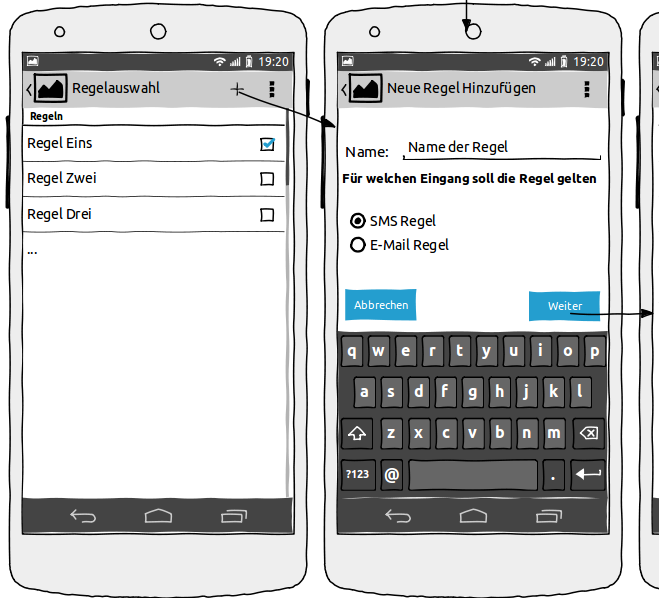
\includegraphics[width=10cm]{Bilder/StartBildschirm.png}
\caption{Wireframe des StartBildschirms mit der Erstellung einer Regel}
\label{Wireframe StartBildschirm}
\vspace{-20pt}
\end{wrapfigure}
App abgebildet, welcher bei Start der App angezeigt werden soll. Hier hat der Nutzer eine \"Ubersicht \"uber alle
\FloatBarrier
\subsection{Die Evaluierung}

\subsection{Die Wireframes nach der Evaluierung}

\subsection{Auswirkungen der Evaluierung auf das Lastenheft}